% =============================================================================
%  Manuscript for J. Chem. Inf. Model. (ACS, achemso). Supporting Information in si.tex.
%  Build:  pdflatex si && pdflatex jcim && bibtex jcim && pdflatex jcim && pdflatex jcim
%  (si first: S-numbered references are imported through xr). Every number comes from the
%  numeros*.tex files written by the analysis scripts (see ../actualizar.sh).
%  main.tex keeps the earlier Elsevier version for reference.
% =============================================================================
\documentclass[journal=jcisd8,manuscript=article,email=true]{achemso}
\usepackage[T1]{fontenc}
\usepackage{amsmath,amssymb}
\usepackage{booktabs}
\usepackage{array}
\usepackage{graphicx}
\usepackage{siunitx}
\usepackage{xcolor}
\usepackage{enumitem}
\usepackage[section]{placeins}
\usepackage{xr-hyper}
\usepackage{hyperref}
\usepackage[capitalise]{cleveref}
\externaldocument{si}
\makeatletter\AtBeginDocument{\def\NAT@cmprs{\z@}}\makeatother   % citas 7, 8, 9 en lugar de un rango con guion
% Macros compartidas por jcim.tex (manuscrito) y si.tex (Supporting Information).
% Todas las cifras proceden de los ficheros numeros*.tex generados por los scripts; no se escriben a mano.
% Generado por hacer_numeros.py a partir de resultados/preliminar.json. No editar a mano.
\newcommand{\nShort}{6{,}137}
\newcommand{\nLong}{133}
\newcommand{\nTotal}{6{,}270}
\newcommand{\betaShortMed}{0.43}
\newcommand{\betaShortLo}{0.26}
\newcommand{\betaShortHi}{0.60}
\newcommand{\betaShortSubPct}{97.8}
\newcommand{\betaShortDiffPct}{0.03}
\newcommand{\betaShortDiffN}{2}
\newcommand{\betaLongMed}{0.65}
\newcommand{\betaLongLo}{0.49}
\newcommand{\betaLongHi}{0.83}
\newcommand{\betaLongSubPct}{69.2}
\newcommand{\betaLongDiffPct}{3.8}
\newcommand{\betaLongDiffN}{5}
\newcommand{\epSd}{0.19}
\newcommand{\epFactor}{1.21}
\newcommand{\epOutOnePointFivePct}{5.4}
\newcommand{\epOutTwoPct}{0.2}
\newcommand{\epRho}{0.92}
\newcommand{\ratioHalf}{8.86}
\newcommand{\ratioHalfLo}{4.70}
\newcommand{\ratioHalfHi}{12.47}
\newcommand{\rhoHalf}{0.91}
\newcommand{\withinHalfPct}{0.0}
\newcommand{\ratioOne}{5.23}
\newcommand{\ratioOneLo}{3.12}
\newcommand{\ratioOneHi}{7.26}
\newcommand{\rhoOne}{0.92}
\newcommand{\withinOnePct}{0.0}
\newcommand{\ratioTwo}{3.34}
\newcommand{\ratioTwoLo}{2.15}
\newcommand{\ratioTwoHi}{4.32}
\newcommand{\rhoTwo}{0.94}
\newcommand{\withinTwoPct}{0.0}
\newcommand{\ratioFive}{1.95}
\newcommand{\ratioFiveLo}{1.47}
\newcommand{\ratioFiveHi}{2.40}
\newcommand{\rhoFive}{0.96}
\newcommand{\withinFivePct}{0.8}
\newcommand{\ratioTen}{1.40}
\newcommand{\ratioTenLo}{1.18}
\newcommand{\ratioTenHi}{1.63}
\newcommand{\rhoTen}{0.98}
\newcommand{\withinTenPct}{16.5}
\newcommand{\ratioFifteen}{1.19}
\newcommand{\ratioFifteenLo}{1.08}
\newcommand{\ratioFifteenHi}{1.31}
\newcommand{\rhoFifteen}{0.99}
\newcommand{\withinFifteenPct}{73.7}
\newcommand{\ratioTwenty}{1.07}
\newcommand{\ratioTwentyLo}{1.03}
\newcommand{\ratioTwentyHi}{1.12}
\newcommand{\rhoTwenty}{1.00}
\newcommand{\withinTwentyPct}{100.0}
\newcommand{\nPairs}{133}
\newcommand{\PairEndRatio}{2.90}
\newcommand{\PairEndLo}{1.58}
\newcommand{\PairEndHi}{4.74}
\newcommand{\PairEndRho}{0.84}
\newcommand{\PairEndRecall}{85}
\newcommand{\PairAvgRatio}{3.90}
\newcommand{\PairAvgLo}{2.14}
\newcommand{\PairAvgHi}{6.22}
\newcommand{\PairAvgRho}{0.85}
\newcommand{\PairAvgRecall}{81}
\newcommand{\nLongLit}{37}
\newcommand{\nLongScreen}{96}
\newcommand{\nRep}{94}
\newcommand{\sdLong}{0.98}
\newcommand{\RepEndRho}{0.48}
\newcommand{\RepEndFactor}{1.43}
\newcommand{\RepEndSd}{0.35}
\newcommand{\RepEndDiffPct}{38}
\newcommand{\RepEndIcc}{0.47}
\newcommand{\RepEndSdAll}{0.49}
\newcommand{\RepEndSdSub}{0.44}
\newcommand{\RepAvgRho}{0.56}
\newcommand{\RepAvgFactor}{1.32}
\newcommand{\RepAvgSd}{0.28}
\newcommand{\RepAvgDiffPct}{32}
\newcommand{\RepAvgIcc}{0.58}
\newcommand{\RepAvgSdAll}{0.43}
\newcommand{\RepAvgSdSub}{0.40}
\newcommand{\RepBetaSd}{0.15}
\newcommand{\RepBetaRho}{-0.07}
\newcommand{\nPrefix}{133}
\newcommand{\valMaxDev}{5e-7}
\newcommand{\driftMed}{1.2}
\newcommand{\driftMax}{34}
\newcommand{\driftFracPct}{63}
\newcommand{\preEndRatioTwo}{4.43}
\newcommand{\preEndErrTwo}{4.43}
\newcommand{\preEndCovTwo}{1}
\newcommand{\preEndRatioFive}{2.83}
\newcommand{\preEndErrFive}{2.83}
\newcommand{\preEndCovFive}{3}
\newcommand{\preEndRatioTen}{2.02}
\newcommand{\preEndErrTen}{2.02}
\newcommand{\preEndCovTen}{14}
\newcommand{\preEndRatioTwenty}{1.43}
\newcommand{\preEndErrTwenty}{1.45}
\newcommand{\preEndCovTwenty}{47}
\newcommand{\preHalfRatioTwo}{6.39}
\newcommand{\preHalfErrTwo}{6.39}
\newcommand{\preHalfCovTwo}{0}
\newcommand{\preHalfRatioFive}{4.05}
\newcommand{\preHalfErrFive}{4.05}
\newcommand{\preHalfCovFive}{0}
\newcommand{\preHalfRatioTen}{2.55}
\newcommand{\preHalfErrTen}{2.55}
\newcommand{\preHalfCovTen}{2}
\newcommand{\preHalfRatioTwenty}{1.78}
\newcommand{\preHalfErrTwenty}{1.78}
\newcommand{\preHalfCovTwenty}{12}
\newcommand{\preFitRatioTwo}{2.83}
\newcommand{\preFitErrTwo}{2.85}
\newcommand{\preFitCovTwo}{23}
\newcommand{\preFitRatioFive}{2.02}
\newcommand{\preFitErrFive}{2.02}
\newcommand{\preFitCovFive}{39}
\newcommand{\preFitRatioTen}{1.48}
\newcommand{\preFitErrTen}{1.51}
\newcommand{\preFitCovTen}{56}
\newcommand{\preFitRatioTwenty}{1.16}
\newcommand{\preFitErrTwenty}{1.24}
\newcommand{\preFitCovTwenty}{78}
\newcommand{\prePowRatioTwo}{0.72}
\newcommand{\prePowErrTwo}{1.50}
\newcommand{\prePowCovTwo}{59}
\newcommand{\prePowRatioFive}{0.95}
\newcommand{\prePowErrFive}{1.37}
\newcommand{\prePowCovFive}{68}
\newcommand{\prePowRatioTen}{1.07}
\newcommand{\prePowErrTen}{1.26}
\newcommand{\prePowCovTen}{74}
\newcommand{\prePowRatioTwenty}{1.11}
\newcommand{\prePowErrTwenty}{1.20}
\newcommand{\prePowCovTwenty}{74}
\newcommand{\ruleBetaNineStopPct}{3}
\newcommand{\ruleBetaNineTime}{49.3}
\newcommand{\ruleBetaNineErr}{1.37}
\newcommand{\ruleBetaNineErrStop}{1.38}
\newcommand{\ruleBetaNineTimeStop}{26.8}
\newcommand{\ruleBetaEightStopPct}{19}
\newcommand{\ruleBetaEightTime}{44.6}
\newcommand{\ruleBetaEightErr}{1.39}
\newcommand{\ruleBetaEightErrStop}{1.39}
\newcommand{\ruleBetaEightTimeStop}{21.2}
\newcommand{\ruleCvTenStopPct}{2}
\newcommand{\ruleCvTenTime}{49.3}
\newcommand{\ruleCvTenErr}{1.37}
\newcommand{\ruleCvTenErrStop}{1.36}
\newcommand{\ruleCvTenTimeStop}{21.0}
\newcommand{\ruleCvTwentyStopPct}{80}
\newcommand{\ruleCvTwentyTime}{15.6}
\newcommand{\ruleCvTwentyErr}{1.79}
\newcommand{\ruleCvTwentyErrStop}{2.22}
\newcommand{\ruleCvTwentyTimeStop}{7.3}
\newcommand{\ruleCvPowStopPct}{24}
\newcommand{\ruleCvPowTime}{43.4}
\newcommand{\ruleCvPowErr}{1.04}
\newcommand{\ruleCvPowErrStop}{1.13}
\newcommand{\ruleCvPowTimeStop}{22.7}
\newcommand{\sensLongSubMinPct}{46}
\newcommand{\sensLongSubMaxPct}{81}
\newcommand{\sensLongDiffMinN}{0}
\newcommand{\sensLongDiffMaxN}{19}
\newcommand{\RepEndIccLo}{0.31}
\newcommand{\RepEndIccHi}{0.63}
\newcommand{\RepEndIccSub}{0.53}
\newcommand{\RepEndIccSubLo}{0.33}
\newcommand{\RepEndIccSubHi}{0.66}
\newcommand{\RepEndPairFactor}{1.65}
\newcommand{\RepEndPairFactorNinetyFive}{2.67}
\newcommand{\RepAvgIccLo}{0.45}
\newcommand{\RepAvgIccHi}{0.70}
\newcommand{\RepAvgIccSub}{0.62}
\newcommand{\RepAvgIccSubLo}{0.45}
\newcommand{\RepAvgIccSubHi}{0.74}
\newcommand{\RepAvgPairFactor}{1.48}
\newcommand{\RepAvgPairFactorNinetyFive}{2.16}
\newcommand{\PairEndRhoLo}{0.76}
\newcommand{\PairEndRhoHi}{0.90}
\newcommand{\PairEndRhoScreen}{0.68}
\newcommand{\PairEndRhoLit}{0.93}
\newcommand{\PairEndTopFiveK}{7}
\newcommand{\PairEndTopFiveHits}{7}
\newcommand{\PairEndTopTenK}{13}
\newcommand{\PairEndTopTenHits}{11}
\newcommand{\PairEndTopTwentyK}{27}
\newcommand{\PairEndTopTwentyHits}{23}
\newcommand{\PairAvgRhoLo}{0.77}
\newcommand{\PairAvgRhoHi}{0.90}
\newcommand{\PairAvgRhoScreen}{0.70}
\newcommand{\PairAvgRhoLit}{0.94}
\newcommand{\PairAvgTopFiveK}{7}
\newcommand{\PairAvgTopFiveHits}{6}
\newcommand{\PairAvgTopTenK}{13}
\newcommand{\PairAvgTopTenHits}{10}
\newcommand{\PairAvgTopTwentyK}{27}
\newcommand{\PairAvgTopTwentyHits}{22}

% Generado por referencias.py a partir de resultados/referencias.json. No editar a mano.
\newcommand{\refN}{133}
\newcommand{\refSlopeVsDapp}{0.70}
\newcommand{\refPowErrMin}{1.33}
\newcommand{\refPowErrMax}{1.45}
\newcommand{\refPowBiasMin}{0.83}
\newcommand{\refPowBiasMax}{1.06}
\newcommand{\refEndErrMin}{2.37}
\newcommand{\refEndErrMax}{3.27}
\newcommand{\refEndBiasMin}{2.37}
\newcommand{\refEndBiasMax}{3.27}
\newcommand{\refFitErrMin}{1.80}
\newcommand{\refFitErrMax}{2.33}
\newcommand{\refFitBiasMin}{1.73}
\newcommand{\refFitBiasMax}{2.33}
\newcommand{\refPowSlopeErrFive}{1.99}
\newcommand{\refPowSlopeRatioFive}{0.54}
\newcommand{\refBracketFivePct}{78}
\newcommand{\refPowSlopeErrTen}{1.52}
\newcommand{\refPowSlopeRatioTen}{0.68}
\newcommand{\refBracketTenPct}{73}
\newcommand{\refPowSlopeErrTwenty}{1.36}
\newcommand{\refPowSlopeRatioTwenty}{0.77}
\newcommand{\refBracketTwentyPct}{69}
\newcommand{\refEndSlopeErrFive}{4.01}
\newcommand{\refFitSlopeErrFive}{3.05}

% Generado por frontera.py a partir de resultados/frontera.json. No editar a mano.
\newcommand{\frN}{133}
\newcommand{\frSplits}{500}
\newcommand{\frMinFixEndOneFive}{20.0}
\newcommand{\frTestFixEndOneFive}{20.0}
\newcommand{\frMetFixEndOneFive}{97}
\newcommand{\frMinFixFitOneFive}{12.0}
\newcommand{\frTestFixFitOneFive}{12.0}
\newcommand{\frMetFixFitOneFive}{61}
\newcommand{\frMinFixPowOneFive}{2.0}
\newcommand{\frTestFixPowOneFive}{2.0}
\newcommand{\frMetFixPowOneFive}{59}
\newcommand{\frMinRegimeOneFive}{34.7}
\newcommand{\frTestRegimeOneFive}{35.2}
\newcommand{\frMetRegimeOneFive}{64}
\newcommand{\frMinPrecFitOneFive}{36.2}
\newcommand{\frTestPrecFitOneFive}{37.0}
\newcommand{\frMetPrecFitOneFive}{67}
\newcommand{\frMinPrecPowOneFive}{11.5}
\newcommand{\frTestPrecPowOneFive}{11.9}
\newcommand{\frMetPrecPowOneFive}{76}
\newcommand{\frMinFixEndOneThree}{30.0}
\newcommand{\frTestFixEndOneThree}{30.0}
\newcommand{\frMetFixEndOneThree}{84}
\newcommand{\frMinFixFitOneThree}{20.0}
\newcommand{\frTestFixFitOneThree}{20.0}
\newcommand{\frMetFixFitOneThree}{96}
\newcommand{\frMinFixPowOneThree}{10.0}
\newcommand{\frTestFixPowOneThree}{7.5}
\newcommand{\frMetFixPowOneThree}{45}
\newcommand{\frMinRegimeOneThree}{n/a}
\newcommand{\frTestRegimeOneThree}{n/a}
\newcommand{\frMetRegimeOneThree}{0}
\newcommand{\frMinPrecFitOneThree}{n/a}
\newcommand{\frTestPrecFitOneThree}{50.0}
\newcommand{\frMetPrecFitOneThree}{0}
\newcommand{\frMinPrecPowOneThree}{21.0}
\newcommand{\frTestPrecPowOneThree}{20.9}
\newcommand{\frMetPrecPowOneThree}{93}
\newcommand{\frMinFixEndOneTwo}{40.0}
\newcommand{\frTestFixEndOneTwo}{40.0}
\newcommand{\frMetFixEndOneTwo}{79}
\newcommand{\frMinFixFitOneTwo}{n/a}
\newcommand{\frTestFixFitOneTwo}{25.0}
\newcommand{\frMetFixFitOneTwo}{0}
\newcommand{\frMinFixPowOneTwo}{20.0}
\newcommand{\frTestFixPowOneTwo}{20.0}
\newcommand{\frMetFixPowOneTwo}{50}
\newcommand{\frMinRegimeOneTwo}{n/a}
\newcommand{\frTestRegimeOneTwo}{n/a}
\newcommand{\frMetRegimeOneTwo}{0}
\newcommand{\frMinPrecFitOneTwo}{n/a}
\newcommand{\frTestPrecFitOneTwo}{n/a}
\newcommand{\frMetPrecFitOneTwo}{0}
\newcommand{\frMinPrecPowOneTwo}{21.0}
\newcommand{\frTestPrecPowOneTwo}{21.1}
\newcommand{\frMetPrecPowOneTwo}{71}

% Generado por techo.py a partir de resultados/techo.json. No editar a mano.
\newcommand{\techoNRep}{94}
\newcommand{\techoNPairsScreen}{96}
\newcommand{\techoEndCorr}{0.69}
\newcommand{\techoEndCorrLo}{0.56}
\newcommand{\techoEndCorrHi}{0.79}
\newcommand{\techoEndRTwo}{0.47}
\newcommand{\techoEndRelTwo}{0.64}
\newcommand{\techoEndRelFour}{0.78}
\newcommand{\techoEndRepForEight}{5}
\newcommand{\techoEndSdDyn}{0.24}
\newcommand{\techoEndSdStruct}{0.26}
\newcommand{\techoEndFracStructPct}{55}
\newcommand{\techoEndFracStructLo}{31}
\newcommand{\techoEndFracStructHi}{72}
\newcommand{\techoEndShortPrefRatio}{1.00}
\newcommand{\techoEndHetRho}{-0.26}
\newcommand{\techoEndHetP}{0.01}
\newcommand{\techoEndSdSlow}{0.40}
\newcommand{\techoEndSdFast}{0.30}
\newcommand{\techoEndRecallOneTopFive}{38}
\newcommand{\techoEndRecallOneTopTen}{45}
\newcommand{\techoEndRecallOneTopTwenty}{56}
\newcommand{\techoEndRecallTwoTopFive}{49}
\newcommand{\techoEndRecallTwoTopTen}{56}
\newcommand{\techoEndRecallTwoTopTwenty}{64}
\newcommand{\techoEndRecallFourTopFive}{61}
\newcommand{\techoEndRecallFourTopTen}{66}
\newcommand{\techoEndRecallFourTopTwenty}{73}
\newcommand{\techoEndRecallOneTopTenLo}{36}
\newcommand{\techoEndRecallOneTopTenHi}{55}
\newcommand{\techoEndDynN}{96}
\newcommand{\techoEndJointN}{92}
\newcommand{\techoEndJointDiffCorr}{0.53}
\newcommand{\techoEndJointFracStructPct}{57}
\newcommand{\techoEndJointFracStructLo}{44}
\newcommand{\techoEndJointFracStructHi}{69}
\newcommand{\techoEndBatchRepRatio}{1.05}
\newcommand{\techoEndBatchRepP}{0.31}
\newcommand{\techoEndBatchRepRatioLo}{0.95}
\newcommand{\techoEndBatchRepRatioHi}{1.17}
\newcommand{\techoEndBatchPrefRatio}{1.00}
\newcommand{\techoEndBatchPrefP}{0.89}
\newcommand{\techoEndBatchPrefRatioLo}{0.93}
\newcommand{\techoEndBatchPrefRatioHi}{1.06}
\newcommand{\techoEndBatchSdOrig}{0.50}
\newcommand{\techoEndBatchSdRep}{0.53}
\newcommand{\techoEndBatchSdOther}{0.47}
\newcommand{\techoEndBatchLeveneP}{0.67}
\newcommand{\techoEndRelUncentred}{0.47}
\newcommand{\techoAvgCorr}{0.76}
\newcommand{\techoAvgCorrLo}{0.66}
\newcommand{\techoAvgCorrHi}{0.84}
\newcommand{\techoAvgRTwo}{0.58}
\newcommand{\techoAvgRelTwo}{0.73}
\newcommand{\techoAvgRelFour}{0.84}
\newcommand{\techoAvgRepForEight}{3}
\newcommand{\techoAvgSdDyn}{0.20}
\newcommand{\techoAvgSdStruct}{0.20}
\newcommand{\techoAvgFracStructPct}{51}
\newcommand{\techoAvgFracStructLo}{20}
\newcommand{\techoAvgFracStructHi}{69}
\newcommand{\techoAvgShortPrefRatio}{0.96}
\newcommand{\techoAvgHetRho}{-0.23}
\newcommand{\techoAvgHetP}{0.02}
\newcommand{\techoAvgSdSlow}{0.29}
\newcommand{\techoAvgSdFast}{0.26}
\newcommand{\techoAvgRecallOneTopFive}{45}
\newcommand{\techoAvgRecallOneTopTen}{52}
\newcommand{\techoAvgRecallOneTopTwenty}{61}
\newcommand{\techoAvgRecallTwoTopFive}{56}
\newcommand{\techoAvgRecallTwoTopTen}{63}
\newcommand{\techoAvgRecallTwoTopTwenty}{70}
\newcommand{\techoAvgRecallFourTopFive}{67}
\newcommand{\techoAvgRecallFourTopTen}{72}
\newcommand{\techoAvgRecallFourTopTwenty}{77}
\newcommand{\techoAvgRecallOneTopTenLo}{44}
\newcommand{\techoAvgRecallOneTopTenHi}{60}
\newcommand{\techoAvgDynN}{96}
\newcommand{\techoAvgJointN}{92}
\newcommand{\techoAvgJointDiffCorr}{0.51}
\newcommand{\techoAvgJointFracStructPct}{52}
\newcommand{\techoAvgJointFracStructLo}{33}
\newcommand{\techoAvgJointFracStructHi}{66}
\newcommand{\techoAvgBatchRepRatio}{1.04}
\newcommand{\techoAvgBatchRepP}{0.34}
\newcommand{\techoAvgBatchRepRatioLo}{0.96}
\newcommand{\techoAvgBatchRepRatioHi}{1.12}
\newcommand{\techoAvgBatchPrefRatio}{0.95}
\newcommand{\techoAvgBatchPrefP}{0.10}
\newcommand{\techoAvgBatchPrefRatioLo}{0.91}
\newcommand{\techoAvgBatchPrefRatioHi}{1.01}
\newcommand{\techoAvgBatchSdOrig}{0.45}
\newcommand{\techoAvgBatchSdRep}{0.46}
\newcommand{\techoAvgBatchSdOther}{0.41}
\newcommand{\techoAvgBatchLeveneP}{0.82}
\newcommand{\techoAvgRelUncentred}{0.58}

% Generado por asignacion.py a partir de resultados/asignacion.json. No editar a mano.
\newcommand{\alN}{6{,}137}
\newcommand{\alReps}{200}
\newcommand{\alKurt}{0.13}
\newcommand{\alShapiroP}{0.81}
\newcommand{\alUnifTopOneBOne}{32}
\newcommand{\alUnifTopOneBTwo}{52}
\newcommand{\alHalvingTopOneBTwo}{85}
\newcommand{\alBoundTopOneBTwo}{82}
\newcommand{\alUnifTopOneBFour}{67}
\newcommand{\alHalvingTopOneBFour}{90}
\newcommand{\alBoundTopOneBFour}{89}
\newcommand{\alEqTopOneUnifTwo}{1.1}
\newcommand{\alSavingTopOneUnifTwo}{1.7}
\newcommand{\alEqTopOneUnifThree}{1.2}
\newcommand{\alSavingTopOneUnifThree}{2.5}
\newcommand{\alEqTopOneUnifFour}{1.2}
\newcommand{\alSavingTopOneUnifFour}{3.2}
\newcommand{\alUnifTopFiveBOne}{41}
\newcommand{\alUnifTopFiveBTwo}{57}
\newcommand{\alHalvingTopFiveBTwo}{77}
\newcommand{\alBoundTopFiveBTwo}{77}
\newcommand{\alUnifTopFiveBFour}{70}
\newcommand{\alHalvingTopFiveBFour}{85}
\newcommand{\alBoundTopFiveBFour}{86}
\newcommand{\alEqTopFiveUnifTwo}{1.2}
\newcommand{\alSavingTopFiveUnifTwo}{1.7}
\newcommand{\alEqTopFiveUnifThree}{1.3}
\newcommand{\alSavingTopFiveUnifThree}{2.2}
\newcommand{\alEqTopFiveUnifFour}{1.5}
\newcommand{\alSavingTopFiveUnifFour}{2.7}
\newcommand{\alUnifTopTenBOne}{48}
\newcommand{\alUnifTopTenBTwo}{61}
\newcommand{\alHalvingTopTenBTwo}{73}
\newcommand{\alBoundTopTenBTwo}{75}
\newcommand{\alUnifTopTenBFour}{72}
\newcommand{\alHalvingTopTenBFour}{83}
\newcommand{\alBoundTopTenBFour}{84}
\newcommand{\alEqTopTenUnifTwo}{1.2}
\newcommand{\alSavingTopTenUnifTwo}{1.6}
\newcommand{\alEqTopTenUnifThree}{1.5}
\newcommand{\alSavingTopTenUnifThree}{2.0}
\newcommand{\alEqTopTenUnifFour}{1.8}
\newcommand{\alSavingTopTenUnifFour}{2.2}
\newcommand{\alBoundHomoTopTenBFour}{85}
\newcommand{\alSavingTopTenUnifFourEmpEnd}{2.2}
\newcommand{\alSavingTopTenUnifFourNormAvg}{2.4}
\newcommand{\alHalvingTopOneBOneQuarterEnd}{74}
\newcommand{\alBoundTopOneBOneQuarterEnd}{68}
\newcommand{\alHalvingTopOneBFourAvg}{84}
\newcommand{\alBoundTopOneBFourAvg}{89}
\newcommand{\alMCErrMax}{0.4}
\newcommand{\alMCErrMed}{0.1}
\newcommand{\alRelPlanLo}{0.31}
\newcommand{\alRelPlanHi}{0.62}
\newcommand{\alRelTrue}{0.47}
\newcommand{\alMisLoTopOneBTwo}{78}
\newcommand{\alMisLoTopOneBFour}{85}
\newcommand{\alMisLoSavingTopOne}{3.0}
\newcommand{\alMisHiTopOneBTwo}{83}
\newcommand{\alMisHiTopOneBFour}{90}
\newcommand{\alMisHiSavingTopOne}{3.2}
\newcommand{\alTwoStageTopOneBTwo}{80}
\newcommand{\alTwoStageTopOneBFour}{85}
\newcommand{\alTwoStageSavingTopOne}{3.2}
\newcommand{\alTwoStageFourkSavingTopOne}{3.0}
\newcommand{\alTwoStageEightkSavingTopOne}{3.2}
\newcommand{\alTrueLoSavingTopOne}{2.4}
\newcommand{\alTrueHiSavingTopOne}{3.2}
\newcommand{\alMisLoTopFiveBTwo}{76}
\newcommand{\alMisLoTopFiveBFour}{85}
\newcommand{\alMisLoSavingTopFive}{2.6}
\newcommand{\alMisHiTopFiveBTwo}{76}
\newcommand{\alMisHiTopFiveBFour}{86}
\newcommand{\alMisHiSavingTopFive}{2.6}
\newcommand{\alTwoStageTopFiveBTwo}{74}
\newcommand{\alTwoStageTopFiveBFour}{80}
\newcommand{\alTwoStageSavingTopFive}{2.4}
\newcommand{\alTwoStageFourkSavingTopFive}{2.4}
\newcommand{\alTwoStageEightkSavingTopFive}{1.9}
\newcommand{\alTrueLoSavingTopFive}{2.1}
\newcommand{\alTrueHiSavingTopFive}{2.9}
\newcommand{\alMisLoTopTenBTwo}{74}
\newcommand{\alMisLoTopTenBFour}{83}
\newcommand{\alMisLoSavingTopTen}{2.2}
\newcommand{\alMisHiTopTenBTwo}{74}
\newcommand{\alMisHiTopTenBFour}{83}
\newcommand{\alMisHiSavingTopTen}{2.1}
\newcommand{\alTwoStageTopTenBTwo}{71}
\newcommand{\alTwoStageTopTenBFour}{80}
\newcommand{\alTwoStageSavingTopTen}{1.8}
\newcommand{\alTwoStageFourkSavingTopTen}{1.8}
\newcommand{\alTwoStageEightkSavingTopTen}{1.3}
\newcommand{\alTrueLoSavingTopTen}{1.8}
\newcommand{\alTrueHiSavingTopTen}{2.5}

% Generado por validacion_asignacion.py. No editar a mano.
\newcommand{\valAlNRep}{94}
\newcommand{\valAlNCamp}{92}
\newcommand{\valAlExtra}{46}
\newcommand{\valAlBrierGainTen}{36}
\newcommand{\valAlCalSlopeTen}{1.10}
\newcommand{\valAlCalSlopeLoTen}{0.66}
\newcommand{\valAlCalSlopeHiTen}{2.27}
\newcommand{\valAlKTen}{9}
\newcommand{\valAlOnlyATen}{67}
\newcommand{\valAlBoundTen}{78}
\newcommand{\valAlRandomTen}{71}
\newcommand{\valAlBothTen}{78}
\newcommand{\valAlDiffLoTen}{-11}
\newcommand{\valAlDiffHiTen}{22}
\newcommand{\valAlBrierGainTwenty}{16}
\newcommand{\valAlCalSlopeTwenty}{0.63}
\newcommand{\valAlCalSlopeLoTwenty}{0.33}
\newcommand{\valAlCalSlopeHiTwenty}{1.36}
\newcommand{\valAlKTwenty}{18}
\newcommand{\valAlOnlyATwenty}{72}
\newcommand{\valAlBoundTwenty}{72}
\newcommand{\valAlRandomTwenty}{70}
\newcommand{\valAlBothTwenty}{72}
\newcommand{\valAlDiffLoTwenty}{-17}
\newcommand{\valAlDiffHiTwenty}{11}

% Generado por ml_demo.py a partir de resultados/ml_demo.json. No editar a mano.
\newcommand{\mlNSys}{6{,}042}
\newcommand{\mlFolds}{5}
\newcommand{\mlCorr}{0.71}
\newcommand{\mlCorrLo}{0.70}
\newcommand{\mlCorrHi}{0.72}
\newcommand{\mlRTwo}{0.50}
\newcommand{\mlFracCeilPct}{103}
\newcommand{\mlImplied}{1.03}
\newcommand{\mlImpliedLo}{1.01}
\newcommand{\mlImpliedHi}{1.00}
\newcommand{\mlRepN}{94}
\newcommand{\mlRepA}{0.67}
\newcommand{\mlRepB}{0.69}
\newcommand{\mlRepMean}{0.78}
\newcommand{\mlRepMeanExp}{0.79}
\newcommand{\mlRepGainLo}{0.07}
\newcommand{\mlRepGainHi}{0.13}
\newcommand{\mlLongN}{133}
\newcommand{\mlLongAllModel}{0.79}
\newcommand{\mlLongAllShort}{0.84}
\newcommand{\mlLongAllDiffLo}{-0.13}
\newcommand{\mlLongAllDiffHi}{0.02}
\newcommand{\mlLongAllN}{133}
\newcommand{\mlLongScreenModel}{0.67}
\newcommand{\mlLongScreenShort}{0.68}
\newcommand{\mlLongScreenDiffLo}{-0.12}
\newcommand{\mlLongScreenDiffHi}{0.13}
\newcommand{\mlLongScreenN}{96}
\newcommand{\mlLongLitModel}{0.67}
\newcommand{\mlLongLitShort}{0.93}
\newcommand{\mlLongLitDiffLo}{-0.47}
\newcommand{\mlLongLitDiffHi}{-0.12}
\newcommand{\mlLongLitN}{37}
\newcommand{\mlLeakN}{168}
\newcommand{\mlLeakTraj}{0.66}
\newcommand{\mlLeakSys}{0.68}

\IfFileExists{numeros_segmentos.tex}{% Generado por segmentos.py a partir de resultados/segmentos.json. No editar a mano.
\newcommand{\segN}{133}
\newcommand{\segEndFirst}{1.63}
\newcommand{\segEndFirstLo}{1.52}
\newcommand{\segEndFirstHi}{1.81}
\newcommand{\segEndFirstVsAll}{1.42}
\newcommand{\segEndFracFirstPct}{93}
\newcommand{\segEndSlope}{0.92}
\newcommand{\segEndFracNegSlopePct}{85}
\newcommand{\segEndWithinTen}{25}
\newcommand{\segEndWilcoxonP}{3.6\times10^{-22}}
\newcommand{\segEndFirstScreen}{1.80}
\newcommand{\segEndFirstLit}{1.28}
\newcommand{\segHalfFirst}{1.47}
\newcommand{\segHalfFirstLo}{1.37}
\newcommand{\segHalfFirstHi}{1.55}
\newcommand{\segHalfFirstVsAll}{1.32}
\newcommand{\segHalfFracFirstPct}{92}
\newcommand{\segHalfSlope}{0.94}
\newcommand{\segHalfFracNegSlopePct}{89}
\newcommand{\segHalfWithinTen}{20}
\newcommand{\segHalfWilcoxonP}{2.0\times10^{-22}}
\newcommand{\segHalfFirstScreen}{1.54}
\newcommand{\segHalfFirstLit}{1.30}
\newcommand{\segBetaFirst}{0.48}
\newcommand{\segBetaLate}{0.31}
\newcommand{\haySegmentos}{1}}{}
\DeclareSIUnit{\angstrom}{\text{\AA}}
\newcommand{\todo}[1]{\textcolor{orange!80!black}{[TODO: #1]}}
\newcommand{\Dapp}{D_{\mathrm{app}}}
\newcommand{\Li}{Li$^{+}$}
\newcommand{\msd}{\mathrm{MSD}}


% Autoría compartida por jcim.tex y si.tex (orden acordado el 2026-10-19).
% Los autores sin afiliación universitaria figuran como "Independent Researcher" con ciudad y país, práctica habitual en ACS.
\author{Francisco Hernando-Gallego}
\email{fhernando@uva.es}
\affiliation{Department of Applied Mathematics, Escuela de Ingenier\'ia Inform\'atica de Segovia,
Universidad de Valladolid, 40005 Segovia, Spain}
\author{Dimitar Vasilev-Vasilev}
\author{Diego Garc\'ia-Santos}
\affiliation{Department of Computer Science, Escuela de Ingenier\'ia Inform\'atica de Segovia,
Universidad de Valladolid, 40005 Segovia, Spain}
\author{Alfonso Campo-Camacho}
\author{Alberto G\'omez-G\'omez}
\affiliation{Independent Researcher, Spain}


\title{Reliability of Short Molecular Dynamics Runs as Screening Labels: Noise Ceilings, Time
Dependence and Adaptive Replicate Allocation}

\abbreviations{MD, MSD, HTP-MD}
\keywords{high-throughput screening, molecular dynamics, label noise, polymer electrolytes,
uncertainty quantification, budget allocation}

\begin{document}

\begin{tocentry}
\centering
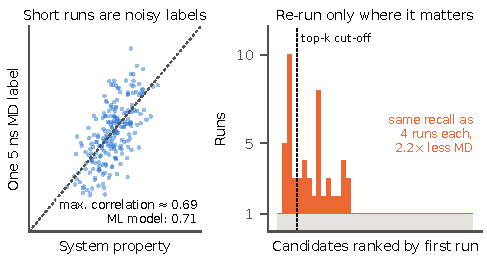
\includegraphics[width=8.25cm]{figures/toc.pdf}
\end{tocentry}

\begin{abstract}
High-throughput molecular dynamics (MD) supplies labels for electrolyte screening and
machine-learning models. Each label, however, comes from one short, noisy run and can depend on
the simulated time. We assess label reliability and simulation-budget allocation using HTP-MD,
the largest public set of polymer
electrolyte trajectories (\nShort{} runs of \SI{5}{\nano\second} and \nLong{} of
\SI{50}{\nano\second}). Only \betaShortDiffN{} short and \betaLongDiffN{} long runs meet an
operational criterion for diffusive lithium motion, the apparent diffusivity at a \SI{5}{\nano\second} lag is
\ratioFive{} times that at \SI{25}{\nano\second}, and the first \SI{5}{\nano\second} of a run
are \segEndFirst{} times faster than its second half, while the polymer is still relaxing,
systematically biasing short labels upwards. From \nRep{} systems simulated twice, a single
\SI{5}{\nano\second} end-point label has reliability \RepEndIcc{} (95\% CI \RepEndIccLo{} to
\RepEndIccHi): no model can correlate with such labels much beyond about \techoEndCorr, a
random forest on monomer fingerprints is indistinguishable from that ceiling (\mlCorr), and
roughly half of the run-to-run noise comes from the initial structure. A short run ranks widely
different polymers well (Spearman \PairEndRhoLit) but not similar ones (\PairEndRhoScreen{} within
the screening set). In simulations with the measured noise, giving further runs only to candidates
whose membership of the top set is uncertain matches four uniform replicates with
\alEqTopTenUnifFour{} runs per candidate for the top 10\% and \alEqTopOneUnifFour{} for the top
1\%; a check on real runs is consistent but underpowered. A decision guide and all code are
provided.
\end{abstract}

% =============================================================================
\section{Introduction}\label{sec:intro}
% =============================================================================
Molecular dynamics (MD) is increasingly used not to study one material carefully but to label
thousands of candidates, either to rank them directly or to train machine-learning models that
extend the search~\cite{Xie2022Accelerating}. Solid polymer electrolytes are a representative
case: lithium transport is slaved to the slow segmental dynamics of the
polymer~\cite{Borodin2006PEO,Webb2015Polyester}, so the simulations needed to converge transport
coefficients are long, while the chemical space is large. The HTP-MD platform, the largest public
collection of such simulations, distributes thousands of short runs of \SI{5}{\nano\second} and a
smaller number of \SI{50}{\nano\second} runs, with raw trajectories and derived
properties~\cite{Xie2022Accelerating,Xie2023HTPMD}.

A label obtained this way has two defects that are easy to overlook once it sits in a table.
It is \emph{time dependent}: the self-diffusion coefficient is defined in the long-time limit, a
diffusivity extracted before the mean-squared displacement (MSD) becomes linear is a property of
the observation window~\cite{Maginn2018BestPractices}, and the window of a screening run is short.
It is also \emph{noisy}: the amorphous structure is sampled once, and two runs of the same polymer
from different initial structures can disagree substantially~\cite{Xie2022Accelerating}. The
dataset's authors addressed both defects by training a multi-task graph network on many short and
few long runs, assuming noise independent of the polymer~\cite{Xie2022Accelerating}. Learning from
noisy labels is well studied in machine learning~\cite{Frenay2014LabelNoise}, and the statistics
of diffusion estimates from finite trajectories are well
understood~\cite{He2018Variances,Bullerjahn2020Optimal,McCluskey2025Accurate,McCluskey2024kinisi},
as are best practices for quantifying the sampling uncertainty of MD
observables~\cite{Grossfield2018BestPractices}. That measurement
noise bounds the performance any model can show is also established: for experimental activity
data, the replicate variability sets the maximum correlation or $R^2$ a model can
reach~\cite{Brown2009Skepticism,Kramer2012Ki}, and computational neuroscience estimates the same
bound as a noise ceiling~\cite{LageCastellanos2019NoiseCeiling}. For simulated labels, however,
to our knowledge the noise across a real screening campaign has not been measured, although the
same question has been raised for chemistry datasets in general~\cite{Crusius2025FittingNoise}; its
sources have not been separated,
whether a model actually reaches the resulting ceiling has not been tested, and the noise has not
been used to decide how a fixed simulation budget should be spent. Unlike experimental noise,
simulation noise can be reduced by spending more computation, which turns the ceiling into a
question of allocation.

We answer these questions on HTP-MD without training a corrective model, using three features of
the public collection: \nRep{} screening systems simulated twice from different initial
structures, \nPairs{} systems simulated at both lengths, and the raw long trajectories, which can
be truncated to emulate shorter runs. Our contributions are:
\begin{enumerate}[leftmargin=*,itemsep=2pt]
  \item \textbf{Time dependence of the labels.} A census of all \nTotal{} trajectories, the
        lag dependence of the apparent diffusivity in the long runs, and a slow decrease of lithium
        mobility within each run that makes its beginning faster than its later part and follows
        an incomplete relaxation of the polymer.
  \item \textbf{Reliability and noise ceiling.} The run-to-run noise of a short label, its
        structural and dynamic sources and its dependence on mobility, the ceiling it imposes on
        the performance that any predictor can show against such labels, a machine-learning model
        that comes close to that ceiling, and the ability of one short run to select the best candidates, checked on a
        second property, the anion diffusivity.
  \item \textbf{Spending the budget.} An evaluation of estimators and stopping rules on truncated
        trajectories, and an evaluation, with the measured noise, of known adaptive strategies that
        concentrate replicates on the candidates near the selection cut-off.
  \item \textbf{A decision guide and reproducible code} for each screening purpose.
\end{enumerate}
None of the statistical tools is new; the contribution is to measure, on a real screening
campaign, the quantities they need and to turn them into decisions about how to run and use the
simulations.

% =============================================================================
\section{Methods}\label{sec:methods}
% =============================================================================
\subsection{Data set}\label{sec:data}
We use every trajectory listed by the public HTP-MD web application~\cite{Xie2023HTPMD} on
6 to 9 October 2026: \nTotal{} trajectories of amorphous polymer/LiTFSI systems simulated with the PCFF+ force
field at \SI{353}{\kelvin}, \nShort{} for \SI{5}{\nano\second} and \nLong{} for
\SI{50}{\nano\second} (\cref{si:tab:dataset}). For each trajectory the platform distributes the
MSD curves of \Li{} and of the anion at 100 lags, derived transport properties and the raw
trajectory, with frames every \SI{2}{\pico\second}. The storage paths identify each system. Every
long run has a \SI{5}{\nano\second} run of the same system (\nLongScreen{} screening polymers and
\nLongLit{} taken from the literature), and, as in the original study~\cite{Xie2022Accelerating},
the two runs of such a pair start from the same initial amorphous structure. In addition, \nRep{}
screening systems were simulated twice for \SI{5}{\nano\second} from different initial
structures. Every system contains \tamNIons{} LiTFSI ion pairs at a nominal molality of
\SI{1.5}{\mole\per\kilo\gram}, equilibrated for \SI{5}{\nano\second} before
production~\cite{Xie2022Accelerating}; from the starting structures, the systems have
\tamNAtomsMin{} to \tamNAtomsMax{} atoms (median \tamNAtomsMed) in \tamChainsMin{} to
\tamChainsMax{} polymer chains (median \tamChainsMed), in cubic boxes of \tamBoxMin{} to
\SI{\tamBoxMax}{\nano\metre} side (ion and chain counts verified on \tamNRecount{} complete
structure files).

\subsection{Labels and their time dependence}\label{sec:labels}
For an MSD curve averaged over time origins and ions,
$\msd(\tau)=\langle|\mathbf r_i(t+\tau)-\mathbf r_i(t)|^2\rangle_{i,t}$, we define the apparent
diffusivity $\Dapp(\tau)=\msd(\tau)/6\tau$. The diffusivity distributed by the platform is the
\emph{end-point} estimate $D_{\mathrm{end}}(T)=\langle|\mathbf r_i(T)-\mathbf r_i(0)|^2\rangle_i/6T$,
which uses only the first and last frames~\cite{HTPMDcode}; we also use the origin-averaged
$\Dapp(T/2)$. Diffusion corresponds to a lag-independent $\Dapp$ and an MSD exponent
$\beta=\mathrm d\ln\msd/\mathrm d\ln\tau=1$. We estimate an effective exponent by a least-squares
fit of $\ln\msd$ against $\ln\tau$ over lags between 20\% and 60\% of the run, and call a run
diffusive when $\beta\ge0.9$; this is an operational classification, and its sensitivity to the
window is reported in \cref{si:tab:sens-window}. For the long runs we compute $\Dapp(\tau)$ from
\SI{0.5}{\nano\second} to \SI{25}{\nano\second} and report its ratio to the reference
$\Dapp(\SI{25}{\nano\second})$ and the Spearman correlation of the rankings. The reference is a
finite-lag quantity, not a converged coefficient. To test whether the beginning of a run differs
from its later part, we split each long run into ten consecutive \SI{5}{\nano\second} segments
and compute, from the data of each segment alone, the end-point and origin-averaged estimates and
the effective exponent; each segment is compared with the geometric mean of the segments between
25 and \SI{50}{\nano\second}. In the same segments we follow the mobility of the anion and of
polymer atoms, the potential energy and pressure (production is at constant volume), and the
lithium-anion clusters computed during the simulations (Supporting Information).

\subsection{Noise model, reliability and noise ceiling}\label{sec:noise-method}
All noise statistics are computed on $\ln D$. Following ref~\citenum{Xie2022Accelerating}, we
model each label as a system-level value plus run-specific noise. Here, the system-level value is
the expected \SI{5}{\nano\second} label across initial structures and dynamical realizations. It
can include biases shared by short runs, such as the early slowdown reported below; it is not the
long-time transport coefficient. Thus, the reliability and noise ceiling describe how well
short-run labels can be predicted. A separate, system-dependent bias distinguishes those labels
from the long-time property.
For the replicated systems, the standard deviation of the difference between the two runs divided
by $\sqrt2$ estimates the noise $\sigma_{\mathrm{run}}$ of one run. With $\sigma_{\mathrm{tot}}$ the
spread of all short runs, the reliability of one run is
\begin{equation}
  r = 1-\sigma_{\mathrm{run}}^2/\sigma_{\mathrm{tot}}^2,
  \label{eq:reliability}
\end{equation}
the fraction of the variance between candidates that reflects differences between systems. We
also report the one-way intraclass correlation computed within the replicated subset. A predictor
that recovered the property of every system exactly would correlate with one label at most
$\sqrt r$ and explain at most a fraction $r$ of its variance, the bound used for experimental
data~\cite{Brown2009Skepticism,Kramer2012Ki} and known as the noise ceiling in computational
neuroscience~\cite{LageCastellanos2019NoiseCeiling}; the mean of $n$ runs has
reliability $nr/[1+(n-1)r]$~\cite{Spearman1910,Brown1910}. To translate reliability into
selection we simulate Gaussian populations with the measured variances and record the fraction of
the truly best 5\%, 10\% and 20\% recovered when selecting by the mean of $n$ runs.

Two sources of noise are separated under an additive model with independent structural and
dynamic contributions, so the split is a statistical attribution conditional on that model rather
than a causal decomposition. Replicas start from different structures, so their difference
contains structural and dynamic noise. The \SI{5}{\nano\second} run of a pair and the
first \SI{5}{\nano\second} of its long run start from the same structure, so their difference
contains only dynamic noise, $\sigma_{\mathrm{dyn}}$; the two are distinct dynamical realisations
(their labels are not identical), although the platform does not document whether they share any
part of the equilibration. Then
$\sigma_{\mathrm{str}}^2=\sigma_{\mathrm{run}}^2-\sigma_{\mathrm{dyn}}^2$, with $\sigma_{\mathrm{run}}$ from the
\nRep{} replicated systems and $\sigma_{\mathrm{dyn}}$ from the \techoEndDynN{} screening pairs. The short
run of a pair is also the original replica of that system, so the two differences share a run; we
therefore repeat the split on the \techoEndJointN{} systems that have both, resampling them jointly. We test whether the noise
depends on mobility by the rank correlation between the absolute difference of two replicas and
their mean. Intervals throughout are obtained by bootstrap over systems (2000 resamples).

\subsection{Machine-learning demonstration}\label{sec:ml-method}
To compare a real model with the ceiling we predict the end-point $\ln D$ of the original
\SI{5}{\nano\second} run of each system from its monomer alone. The input is the Morgan count
fingerprint (radius 2, 2048 bits; RDKit) of the monomer SMILES distributed by HTP-MD, including
the dummy atoms that mark the connection points, so chain architecture is not represented. The
model is a random forest (scikit-learn; 400 trees, a fraction 0.3 of the features per split, at
least two samples per leaf), with these settings fixed in advance and not tuned. It is trained on
the \mlNSys{} systems that have an original screening run, literature polymers included
(\nOnlyReplica{} system appears only as a replica and is left out), and evaluated by
\mlFolds-fold cross-validation split by system, so that every prediction is out of sample. As a
stricter split we group the monomers into chemical families by Butina clustering of the Tanimoto
distances of their binary Morgan fingerprints, at two similarity thresholds, and keep each family
within one fold. Intervals for the correlations are obtained by bootstrap over systems of the
out-of-fold predictions. To measure the effect of splitting by trajectory instead of by system,
we repeat the cross-validation with every trajectory, including the second runs of the replicated
systems, as its own group, and compare the two splits on the replicated pairs whose two runs fell
in different folds (\mlLeakPairs{} of the \nRep{}; in the other \mlLeakSameFold{} both runs were
in the same test fold).

\subsection{Selection from paired runs}\label{sec:selection-method}
For the \nPairs{} pairs we compare the end-point label of the \SI{5}{\nano\second} run with the
reference of the long run of the same system: median ratio, Spearman correlation (separately for
screening and literature polymers) and the recall of the best 5\%, 10\% and 20\% systems, that is,
the fraction of the $k$ best according to the reference that are also among the $k$ best according
to the short run, against the recall $k/n$ of a random choice. Because the two runs share their
initial structure, this comparison contains only the dynamic part of the noise.

\subsection{Truncated trajectories and stopping rules}\label{sec:stopping-method}
From the raw trajectory of each long run we extract the unwrapped lithium positions, subtract the
centre-of-mass motion of the whole system as the released library does~\cite{HTPMDcode} (validation
in the Supporting Information), truncate the trajectory to its first $T$ nanoseconds and estimate the
diffusivity from that prefix alone with four estimators: the end-point, the origin-averaged
$\Dapp(T/2)$, one sixth of the slope of a linear fit to the MSD over $0.2T$ to $0.5T$, the
conventional procedure~\cite{Maginn2018BestPractices}, and a power law $\msd=A\tau^{\beta}$ fitted
over $0.1T$ to $0.5T$ and extrapolated to $\tau_{\mathrm{ref}}$, $\widehat{\Dapp}=A\tau_{\mathrm{ref}}^{\beta-1}/6$.
Estimates are compared with the reference of the full run through the typical multiplicative error
$\exp(\mathrm{median}\,|\ln(\hat D/D_{\mathrm{ref}})|)$; because the reference shares data with the
prefix, we repeat the comparison against references at other lags and against the late slope of
the MSD. Stopping rules stop a run when its effective exponent reaches a threshold or when the
bootstrap coefficient of variation of an estimate falls below a tolerance; runs that never stop are
simulated to \SI{50}{\nano\second}, and cost and error are averaged over all runs. Thresholds are
chosen on a random half of the systems and evaluated on the other half (\frSplits{} partitions).

\subsection{Adaptive allocation of replicates}\label{sec:allocation-method}
Consider a campaign of $N=\alN$ candidates, a hypothetical population the size of the set of
short runs, with a budget of $b$ \SI{5}{\nano\second} runs per
candidate on average, whose goal is the top $k$. System values are drawn from
$\mathcal N(0,\sigma_{\mathrm{sys}}^2)$ with $\sigma_{\mathrm{sys}}^2=r\sigma_{\mathrm{run}}^2/(1-r)$,
and each run adds noise whose standard deviation varies linearly with mobility so as to reproduce
the measured noise of the slow and fast halves; every replicate starts from a new structure and
carries the full noise. The unit of cost is therefore a complete new-structure run, which in the
HTP-MD protocol comprises \SI{5}{\nano\second} of equilibration and \SI{5}{\nano\second} of
production; budgets and savings below are counted in such runs. A normal prior and a Gaussian approximation
of the posterior, with the noise evaluated at the observed mean of each candidate rather than at
its unknown value, give the mean and uncertainty of each candidate. We compare three allocations of the budget. \emph{Uniform}: $b$ runs for every
candidate. \emph{Successive halving}~\cite{Jamieson2016SuccessiveHalving}: one run for all, then
further runs for the best $4k$, $2k$ and $k$, in rounds that restart from $4k$ until the budget
is spent.
\emph{Boundary-focused}: one run for all, then batches of \alBatchPct\% of $N$ further runs to the
candidates with the largest $p(1-p)$, where $p$ is the posterior probability of lying above the
current top-$k$ cut-off (the $k$-th largest posterior mean, treated as fixed within a batch), in the spirit of optimal computing budget
allocation~\cite{Chen2000OCBA} and of its version for selecting a subset of the best
designs~\cite{Chen2008OCBAm}. The final selection is the top $k$ by posterior mean, and the
metric is the recall of the true top $k$, averaged over \alReps{} simulated campaigns (Monte
Carlo standard error at most \alMCErrMax{} percentage points). As a simple reference we add a
\emph{two-stage re-screening}: one run for all, then the rest of the budget spread evenly over a
fixed shortlist of the best $2k$, $4k$ or $8k$ after the first run, taking for each budget the best
of the three shortlists. Robustness is checked with the empirical shape of the short-run
distribution instead of a normal one, with the origin-averaged label, with a constant instead of
a mobility-dependent noise, with a misestimated reliability (the runs follow the measured noise,
but the allocation and the selection use the ends of its 95\% interval), and with the true
reliability at either end of that interval. The algorithm and its parameters are given in the
Supporting Information.

The public data allow a partial check on real runs. In the replicated systems, the first run is
the original screening run and the second starts from a new structure, and \valAlNCamp{} of them
also have a long run, which starts from the same structure as the first. We use them in two ways,
with noise parameters estimated leaving out the system being evaluated. First, from one run of
each system the model predicts the probability that the other run exceeds the top-$k$ cut-off;
we compare these predictions with what happens (Brier score against the base rate and calibration
slope). Second, we run a small real campaign: every system receives its first run, and
\valAlExtra{} second runs go either to the candidates with the largest $p(1-p)$ or to randomly
chosen ones; the selection is evaluated against the long runs, which are independent of the second
runs.

% =============================================================================
\section{Results and Discussion}\label{sec:results}
% =============================================================================
\subsection{Labels depend on the simulated time}\label{sec:res-time}
After \SI{5}{\nano\second} the median effective exponent of the lithium MSD is \betaShortMed{}
(10th to 90th percentile range \betaShortLo{} to \betaShortHi): \betaShortSubPct\% of the runs have $\beta<0.7$ and
\betaShortDiffN{} of \nShort{} meet the diffusive criterion (\cref{fig:regime}). Ten times more
simulation moves the distribution but does not resolve the problem: at \SI{50}{\nano\second} the
median is \betaLongMed{} and \betaLongDiffN{} of \nLong{} runs are diffusive
(\sensLongDiffMinN{} to \sensLongDiffMaxN{} depending on the fitting window, \cref{si:tab:sens-window}).
In the long runs the apparent diffusivity falls steadily with the lag (\cref{fig:long}): at
\SI{5}{\nano\second} it is a median \ratioFive{} times its value at \SI{25}{\nano\second}
(10th to 90th percentile range \ratioFiveLo{} to \ratioFiveHi), and only \withinFifteenPct\% of the systems are
within 25\% of the reference at \SI{15}{\nano\second} (\cref{si:tab:lag}). Rankings are far more
stable: the Spearman correlation with the ranking at \SI{25}{\nano\second} is \rhoHalf{} already at
\SI{0.5}{\nano\second} and \rhoFive{} at \SI{5}{\nano\second}. A short-run label is therefore an
apparent, window-dependent quantity whose value should not be compared across studies with
different lengths, but whose ordering carries information.

Labels also depend on \emph{when} the time is simulated (\cref{fig:segments}). Analysed with its own
data only, the first \SI{5}{\nano\second} segment of a long run is a median \segEndFirst{} times
faster than the segments between 25 and \SI{50}{\nano\second} (95\% interval \segEndFirstLo{} to
\segEndFirstHi; \segHalfFirst{} with the origin-averaged estimator), and it is faster in
\segEndFracFirstPct\% of the systems (Wilcoxon signed-rank $p=\segEndWilcoxonP$). The slowdown is
not a short transient: the apparent diffusivity keeps falling by a factor of \segEndSlope{} every
\SI{10}{\nano\second} between 5 and \SI{50}{\nano\second}, in \segEndFracNegSlopePct\% of the
systems, and the effective exponent of the segments decreases from \segBetaFirst{} in the first
to \segBetaLate{} in the late ones. Lithium mobility therefore keeps decreasing throughout the
runs, despite the \SI{5}{\nano\second} equilibration that precedes
production~\cite{Xie2022Accelerating}, and the whole system is still relaxing
(\cref{si:tab:slowdown}). At constant volume, the potential energy falls between the first and the
late segments in all \slowN{} systems, by a median \slowPe{}~kcal\,mol$^{-1}$ per atom,
\slowPeOverNoise{} times the fluctuation of its \SI{100}{\pico\second} averages, and the anion
and the polymer slow down with lithium ($\times$\slowTfsi{} and $\times$\slowMat). Across
systems, the slowdown of lithium follows that of the polymer (Spearman \slowCorrMat, 95\%
interval \slowCorrMatLo{} to \slowCorrMatHi) and the relaxation of the energy (\slowCorrPe), but
not the change in ion clustering, which is small and uncorrelated with it (\slowCorrCluster).
The early, faster window is thus consistent with a polymer that has not finished relaxing after the
equilibration, as expected if lithium transport is slaved to segmental
dynamics~\cite{Borodin2006PEO,Webb2015Polyester}; these are correlations, not a demonstration of
cause. Detecting the end of equilibration from the trajectory itself~\cite{Chodera2016Equilibration}
would be a natural way to start production per system.
The effect is stronger for the screening polymers (\segEndFirstScreen) than for those taken from
the literature (\segEndFirstLit).


\begin{figure}[ht]
\centering
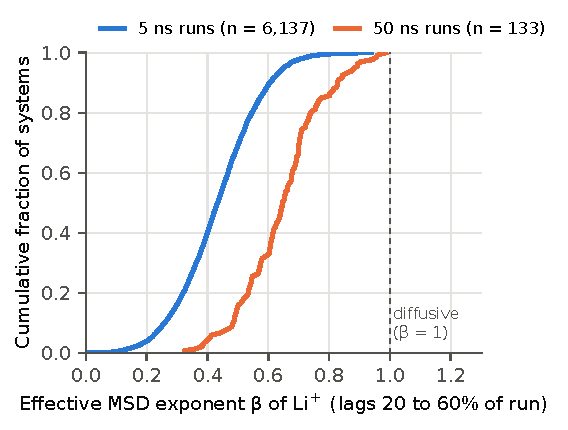
\includegraphics[width=0.5\textwidth]{figures/fig1_exponent_ecdf.pdf}
\caption{Cumulative distribution of the effective MSD exponent $\beta$ of \Li{} in the
\SI{5}{\nano\second} and \SI{50}{\nano\second} runs. The dashed line marks diffusive motion
($\beta=1$); runs are counted as diffusive when $\beta\geq0.9$.}
\label{fig:regime}
\end{figure}

\begin{figure}[ht]
\centering
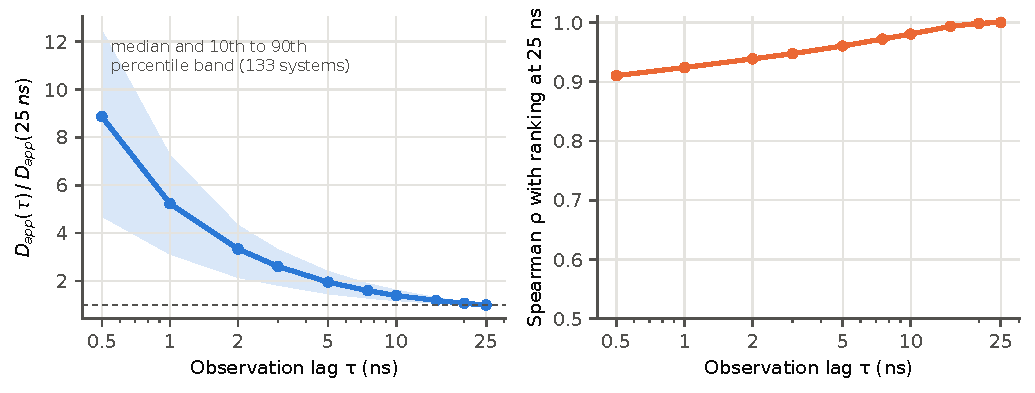
\includegraphics[width=\textwidth]{figures/fig2_long_runs.pdf}
\caption{Lag dependence in the \nLong{} runs of \SI{50}{\nano\second}. Left: apparent
diffusivity of \Li{} relative to its value at \SI{25}{\nano\second} (median and 10th to 90th percentile band).
Right: Spearman correlation between the rankings at lag $\tau$ and at \SI{25}{\nano\second}.}
\label{fig:long}
\end{figure}

\begin{figure}[ht]
\centering
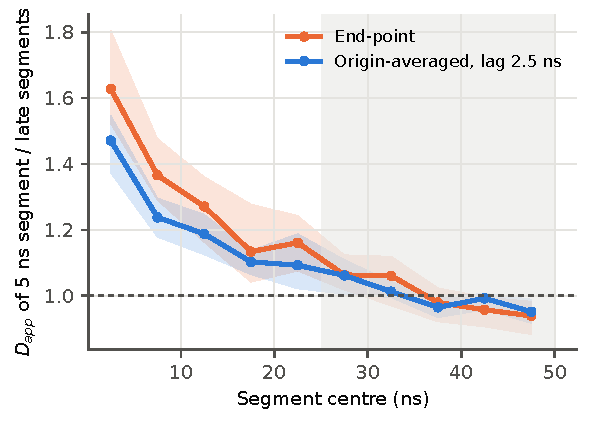
\includegraphics[width=0.6\textwidth]{figures/fig7_segments.pdf}
\caption{Apparent diffusivity of consecutive \SI{5}{\nano\second} segments of the \segN{} long
runs, each computed from its own data, relative to the segments between 25 and
\SI{50}{\nano\second} (shaded): median over systems and 95\% bootstrap interval.}
\label{fig:segments}
\end{figure}

\subsection{Run-to-run noise and its sources}\label{sec:res-noise}
A single \SI{5}{\nano\second} run deviates from the value of its system by a typical factor of
\RepEndFactor{} for the end-point label ($\sigma_{\mathrm{run}}=\RepEndSd$ in log units) and
\RepAvgFactor{} for the origin-averaged one, estimated from pairs of runs of the same system from
different structures (\cref{si:tab:replicas}). Against the spread of the
whole screening set, the reliability of one end-point label is \RepEndIcc{} (95\% interval
\RepEndIccLo{} to \RepEndIccHi), and \RepAvgIcc{} (\RepAvgIccLo{} to \RepAvgIccHi) for the origin-averaged
label; the intraclass correlation within the replicated subset agrees (\RepEndIccSub{} and
\RepAvgIccSub). Roughly half of the variance between screened candidates is therefore noise.

The noise has two comparable sources. The \SI{5}{\nano\second} run of each pair agrees with the
first \SI{5}{\nano\second} of its long run, which starts from the same structure, to a median
ratio of \techoEndShortPrefRatio{} with a noise of \techoEndSdDyn, against \RepEndSd{} between
replicas from different structures: the initial structure accounts for
\techoEndFracStructPct\% (\techoEndFracStructLo{} to \techoEndFracStructHi\%) of the run-to-run variance
and the dynamics for the rest; on the \techoEndJointN{} systems with both comparisons, resampled
jointly, the share is \techoEndJointFracStructPct\% (\techoEndJointFracStructLo{} to
\techoEndJointFracStructHi\%). The originals, the replicas and the long runs were produced in
different batches of the data set, but none is shifted or differently spread
(Supporting Information, after \cref{si:tab:replicas}). Re-sampling the structure and averaging the dynamics both reduce the
noise. A replicate that starts from a new structure samples both sources, as ensembles of
independent runs do in other MD applications~\cite{Coveney2016Ensembles}, but it also costs a new
equilibration. The measured split shows why that cost can be worth paying: even if extending a
single run removed the dynamic noise completely, the structural part would remain, and the
reliability of a label from one structure could not exceed \techoEndOneStructMax, whereas the
mean of two runs from different structures already reaches \techoEndRelTwo. The bound assumes
that the memory of the initial structure does not fade as the run is extended, which these data
cannot test, and a longer run also measures a later, slower window. In the allocation results
below every run, uniform or adaptive, starts from a new structure. The noise
also depends on mobility: it is \techoEndSdSlow{} in the slower half of the replicated systems and
\techoEndSdFast{} in the faster half (rank correlation between the absolute difference and the
level $\techoEndHetRho$, $p=\techoEndHetP$), whereas the learning model of the original study assumes
noise independent of the polymer~\cite{Xie2022Accelerating}. Two candidates measured once each
differ by a factor of \RepEndPairFactor{} from noise alone at one standard deviation and up to
\RepEndPairFactorNinetyFive{} at the 95\% level.

\subsection{A noise ceiling for learned predictors}\label{sec:res-ceiling}
The reliability bounds what any predictor can achieve against short-run labels
(\cref{tab:ceiling}). A model that recovered the property of every system exactly would correlate
with a single end-point label at most \techoEndCorr{} (95\% interval
\techoEndCorrLo{} to \techoEndCorrHi) and explain at most $R^2=\techoEndRTwo$ of its variance; with the
origin-averaged label the ceilings are \techoAvgCorr{} and \techoAvgRTwo. Choosing the best 10\% by
one end-point label recovers \techoEndRecallOneTopTen\% of the truly best tenth, which is also the
apparent recall of a perfect model evaluated against such labels. Averaging runs raises the ceiling:
two end-point runs give a reliability of \techoEndRelTwo, four give \techoEndRelFour, and a
reliability of 0.8 requires \techoEndRepForEight{} runs (\techoAvgRepForEight{} with the
origin-averaged label). The original study estimated that its graph network predicts the
conductivity with the accuracy of about four simulations per polymer~\cite{Xie2022Accelerating};
for the lithium diffusivity studied here, four runs correspond to a reliability of
\techoEndRelFour.

A real model comes close to this ceiling (\cref{tab:ml}). A random forest on Morgan fingerprints
of the monomer, trained on the \mlNSys{} systems with cross-validation split by system
(see Methods), gives out-of-sample predictions that
correlate with the labels with Pearson $r=\mlCorr$ (95\% interval \mlCorrLo{} to \mlCorrHi;
$R^2=\mlRTwo$), statistically indistinguishable from the estimated ceiling of \techoEndCorr{}
(95\% interval \techoEndCorrLo{} to \techoEndCorrHi): the ratio of the two is \mlCeilRatio, and
\mlCeilRatioLo{} to \mlCeilRatioHi{} across the interval of the ceiling, whose uncertainty
dominates. Keeping each chemical family of monomers within one fold barely changes the result: \mlFamFineCorr{} with
\mlFamFineGroups{} families (Tanimoto $\geq\mlFamFineSim$) and \mlFamCoarseCorr{} with
\mlFamCoarseGroups{} (Tanimoto $\geq\mlFamCoarseSim$), although the screened chemistry is narrow:
even then the most similar training monomer has a median similarity of \mlFamCoarseNN, against
\mlNNSys{} when splitting by system, so this tests interpolation within the screened chemistry,
not generalisation to new families. That the point estimate exceeds the ceiling
slightly suggests that the reliability of the whole population is somewhat higher than the
replicated subset indicates; either way, a simple model is already close to what single short-run
labels allow. Being this close to the estimated ceiling makes further improvements by better
architectures hard to demonstrate against single short-run labels, although it does not exclude
them; averaged labels or long-run references would show them more clearly. The replicated
systems are consistent with the measurement model. For the same predictions, the correlation rises from
\mlRepA{} and \mlRepB{} against either single label to \mlRepMean{} against the mean of the two,
as the reliability of a two-run mean predicts (\mlRepMeanExp; gain 95\% interval \mlRepGainLo{}
to \mlRepGainHi). Against such labels, better labels rather than better models are what can
raise the measured performance.

Against the long runs, the model, which never saw these systems, ranks the
\SI{50}{\nano\second} reference as well as the system's own \SI{5}{\nano\second} run among the
screening polymers (Spearman \mlLongScreenModel{} against \mlLongScreenShort), but worse among the
literature polymers (\mlLongLitModel{} against \mlLongLitShort), whose chemistry lies outside
the screened space. Because each long run shares its initial structure with the short run, this
comparison favours the short run; a model trained on short labels is thus a substitute for a short
simulation within the chemical space it was trained on, not beyond it.

Two practical consequences follow. A test metric computed against single short-run labels cannot
exceed the ceiling, so a model close to it is as good as the labels allow, and progress has to be
measured against averaged labels. And because \techoNRep{} systems appear twice in the public
dataset, splits should be made by system; in this dataset the effect of splitting by trajectory
instead is small (\mlLeakTraj{} against \mlLeakSys{} on the \mlLeakN{} trajectories of the
\mlLeakPairs{} replicated pairs split across folds), because the model agrees with either run of a replicated system more closely than the two runs
agree with each other (rank correlation \RepEndRho), so the partner's label adds little.


\begin{table}[ht]
\centering
\caption{Noise ceiling of short-run labels in the screening population: reliability of the mean of
$n$ runs, maximum correlation of a perfect predictor with that label, and recall of the truly best
systems when selecting by it.}\label{tab:ceiling}
{\footnotesize% Generado por techo.py. No editar a mano.
\begin{tabular}{lrrrrrr}
\toprule
 & & & & \multicolumn{3}{c}{Recall of the true top} \\
\cmidrule(lr){5-7}
Label & Runs averaged & Reliability & Max.\ correlation & 5\% & 10\% & 20\% \\
\midrule
End-point & 1 & 0.47 & 0.69 & 38\% & 45\% & 56\% \\
 & 2 & 0.64 & 0.80 & 49\% & 56\% & 64\% \\
 & 3 & 0.73 & 0.85 & 56\% & 63\% & 70\% \\
 & 4 & 0.78 & 0.88 & 61\% & 66\% & 73\% \\
\addlinespace
Origin-averaged, lag $T/2$ & 1 & 0.58 & 0.76 & 45\% & 52\% & 61\% \\
 & 2 & 0.73 & 0.85 & 56\% & 63\% & 70\% \\
 & 3 & 0.80 & 0.90 & 63\% & 68\% & 75\% \\
 & 4 & 0.84 & 0.92 & 67\% & 72\% & 77\% \\
\bottomrule
\end{tabular}
}
\end{table}

\begin{table}[ht]
\centering
\caption{Out-of-sample correlation of a random forest on monomer fingerprints with short-run
labels (cross-validation split by system, or by chemical family of the monomer), against the
noise ceiling of each label. The ceilings and their intervals rest on the run-to-run noise of
the \nRep{} replicated systems, not on the \mlNSys{} systems of the first rows.}\label{tab:ml}
\resizebox{\textwidth}{!}{% Generado por ml_demo.py. No editar a mano.
\begin{tabular}{lrrr}
\toprule
Target of the out-of-sample prediction & Systems & Pearson $r$ (95\% CI) & Ceiling \\
\midrule
One 5 ns label, all systems & 6{,}042 & 0.71 (0.70 to 0.72) & 0.69 \\
One 5 ns label, replicated systems & 94 & 0.68 & 0.69 \\
Mean of two 5 ns labels, replicated systems & 94 & 0.78 (0.66 to 0.86) & 0.80 \\
\bottomrule
\end{tabular}
}
\end{table}

\subsection{Selecting candidates from one short run}\label{sec:res-selection}
For the \nPairs{} systems simulated at both lengths, the end-point label of the
\SI{5}{\nano\second} run is a median \PairEndRatio{} times the long-run reference (10th to 90th percentile range
\PairEndLo{} to \PairEndHi; \cref{si:fig:pairs}), and the Spearman correlation between them is
\PairEndRho{} (95\% interval \PairEndRhoLo{} to \PairEndRhoHi). The correlation owes much to the wide
range of mobilities in this subset: it is \PairEndRhoLit{} among the \nLongLit{} literature
polymers but \PairEndRhoScreen{} among the \nLongScreen{} screening polymers. In the whole
paired set the short run identifies \PairEndTopTenHits{} of the \PairEndTopTenK{} best systems
(\cref{tab:selection}), but these top sets consist almost entirely of literature polymers
(\LitInTopTen{} of \PairEndTopTenK{} and \LitInTopTwenty{} of \PairEndTopTwentyK), which are easy to
separate. Within the \ScrN{} screening polymers the short run still recovers \ScrTopTenHits{} of
the \ScrTopTenK{} best and \ScrTopTwentyHits{} of the \ScrTopTwentyK{} best, against 10\% and 20\%
by chance. These recalls are optimistic, because the short and long runs of a pair share their
initial structure and only the dynamic part of the noise separates them. A short run thus
separates good from poor electrolytes but cannot resolve similar ones, in line with the noise
ceiling above.

The median ratio of \PairEndRatio{} is larger than the \ratioFive{} obtained at the same lag from
the origin-averaged long curves, and this slowdown explains the gap. The short runs behave like the
first \SI{5}{\nano\second} of the long runs (median ratio \techoEndShortPrefRatio), and that
first segment is \segEndFirstVsAll{} times faster than the average of all segments, which is
roughly what separates a single early window from a curve averaged over all time origins. Short
labels in the dataset are therefore systematically biased upwards by the early, faster part of
the trajectory, and more so for the screening polymers. For ranking, this bias matters only to the
extent that it differs between systems.

\begin{table}[ht]
\centering
\caption{Recall of the best systems according to the \SI{50}{\nano\second} reference when they are
selected from the \SI{5}{\nano\second} run of the same system (\nPairs{} systems; the last rows
only the \ScrN{} screening polymers). Intervals by bootstrap over systems; ``Random'' is the expected
recall of a random selection of $k$ systems. All recalls are optimistic, because the two runs of a
pair share their initial structure.}
\label{tab:selection}
% Generado por incertidumbre.py. No editar a mano.
\begin{tabular}{lrrrrr}
\toprule
Estimator, \SI{5}{\nano\second} run & Top & $k$ & Hits & Recall (95\% CI) & Random \\
\midrule
End-point & 5\% & 7 & 7 & 100\% (50 to 100) & 5\% \\
 & 10\% & 13 & 11 & 85\% (62 to 100) & 10\% \\
 & 20\% & 27 & 23 & 85\% (71 to 94) & 20\% \\
Origin-averaged, lag $T/2$ & 5\% & 7 & 6 & 86\% (50 to 100) & 5\% \\
 & 10\% & 13 & 10 & 77\% (62 to 100) & 10\% \\
 & 20\% & 27 & 22 & 81\% (75 to 94) & 20\% \\
End-point, screening only & 5\% & 5 & 4 & 80\% (67 to 100) & 5\% \\
 & 10\% & 10 & 7 & 70\% (50 to 86) & 10\% \\
 & 20\% & 19 & 14 & 74\% (54 to 83) & 20\% \\
\bottomrule
\end{tabular}

\end{table}

\subsection{Spending the budget within a run: estimators and stopping}\label{sec:res-stopping}
When only the first $T$ nanoseconds of a long run are available (\cref{fig:prefix},
\cref{si:tab:prefix}), the end-point, half-lag and linear-fit estimates overestimate the reference
at every short length, by typical factors of \preEndErrFive, \preHalfErrFive{} and \preFitErrFive{}
at \SI{5}{\nano\second}, and their bootstrap intervals seldom contain it (\preEndCovFive\%,
\preHalfCovFive\% and \preFitCovFive\% of the runs): a within-run error bar describes the apparent
diffusivity at the lags available in the prefix, not its distance to the long-lag value. A
power-law extrapolation removes most of the systematic deviation (median ratio \prePowRatioFive,
typical error \prePowErrFive{} from \SI{5}{\nano\second}) but ranks the systems slightly worse
(Spearman \prePowRhoFive{} against \preEndRhoFive{} for the end-point), because it extrapolates an
exponent that is not reproducible between runs, and it underestimates the late slope of the MSD
(median ratio \refPowSlopeRatioFive; \cref{si:tab:sens-prefix-ref}). A power law with $\beta<1$
has no crossover to diffusion: its slope keeps falling with the lag, whereas the true MSD must
eventually become linear. The extrapolation is therefore an empirical estimate of the apparent
diffusivity at a chosen lag within or near the observed window, not of the long-time coefficient.
Adaptive stopping rules, based on the exponent or on the bootstrap precision, do not improve on
the cost-error frontier of fixed-length runs: they either rarely stop early or stop early at the
price of large errors (\cref{si:fig:frontier,si:tab:rules}), and settings chosen on half of the systems often miss their
target on the other half: the power-law length chosen for a typical error of $\times1.3$ meets it
on the held-out systems in only \frMetFixPowOneThree\% of the partitions (\cref{si:tab:frontier}).
Within a run, then, there is little to save; the budget is better spent across candidates.

\begin{figure}[ht]
\centering
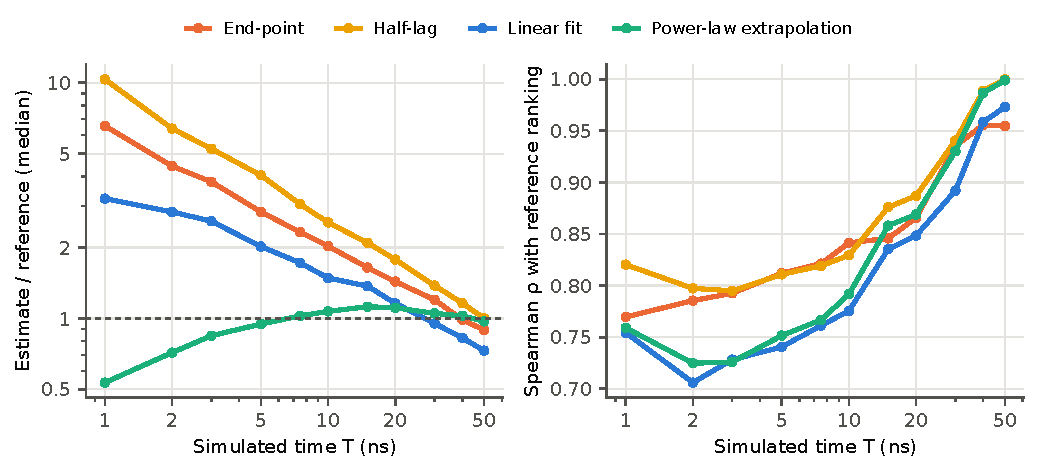
\includegraphics[width=\textwidth]{figures/fig5_prefix_estimators.pdf}
\caption{Estimators computed from the first $T$ nanoseconds of the \nPrefix{} long runs. Left:
median ratio to the reference $\Dapp(\SI{25}{\nano\second})$ of the full run. Right: Spearman
correlation with the reference ranking.}
\label{fig:prefix}
\end{figure}


\subsection{Spending the budget across candidates: adaptive allocation}\label{sec:res-allocation}
The noise model measured above is compatible with the replicated systems: the
differences between replicas show no departure from a Gaussian (excess kurtosis \alKurt,
Shapiro-Wilk $p=\alShapiroP$).
With it, how replicates are distributed matters more than how many are run (\cref{fig:allocation};
values in \cref{si:tab:allocation}). Uniform replicates improve slowly: for the top 10\% of \alN{} candidates
the recall rises from \alUnifTopTenBOne\% with one run to \alUnifTopTenBFour\% with four.
Boundary-focused allocation reaches \alBoundTopTenBTwo\% with two runs per candidate on average
and \alBoundTopTenBFour\% with four, and matches four uniform replicates with
\alEqTopTenUnifFour{} runs per candidate, a saving of $\times$\alSavingTopTenUnifFour. The saving
grows with the selectivity of the target: $\times$\alSavingTopFiveUnifFour{} for the top 5\% and
$\times$\alSavingTopOneUnifFour{} for the top 1\% (\cref{si:tab:alloc-eq}). Successive halving, which re-runs the current leaders in repeated rounds, performs
similarly: with the end-point label it is better for the top 1\% at small budgets
(\alHalvingTopOneBOneQuarterEnd\% against \alBoundTopOneBOneQuarterEnd\% with 1.25 runs per
candidate), and with the origin-averaged label it is worse at larger budgets
(\alHalvingTopOneBFourAvg\% against \alBoundTopOneBFourAvg\% with four).
Even a two-stage re-screening, in which the budget left after the first run is spread evenly over
a fixed shortlist of the best candidates, captures most of the gain: with a shortlist of the best $4k$ fixed in advance it saves
$\times$\alTwoStageFourkSavingTopOne{} for the top 1\%, $\times$\alTwoStageFourkSavingTopFive{}
for the top 5\% and $\times$\alTwoStageFourkSavingTopTen{} for the top 10\%, and the best of three
shortlist sizes, chosen in hindsight, adds little ($\times$\alTwoStageSavingTopOne,
$\times$\alTwoStageSavingTopFive{} and $\times$\alTwoStageSavingTopTen). Most of the saving therefore comes from not
spending replicates on candidates that the first run already places far from the cut-off;
allocating them where the selection is still in doubt adds the rest, and does so without a
shortlist size to tune. The price is sequential work: in batches of \alBatchPct\% of the
candidates, matching four uniform replicates takes \alRoundsTopTen{} rounds of simulation and
analysis for the top 10\% and \alRoundsTopOne{} for the top 1\%, against a single extra round
for the two-stage re-screening. Where each round waits in a queue, the two-stage scheme is the
practical choice, and its loss is small for the most selective targets. Nor does the saving depend on knowing the
reliability exactly: planning with $r=\alRelPlanLo$ or $\alRelPlanHi$ instead of \alRelTrue{} gives
savings of $\times$\alMisLoSavingTopTen{} and $\times$\alMisHiSavingTopTen{} for the top 10\%
(\cref{si:tab:alloc-checks}), and if the true reliability lies at either end of its interval the
saving is $\times$\alTrueLoSavingTopTen{} to $\times$\alTrueHiSavingTopTen{} for the top 10\% and
$\times$\alTrueLoSavingTopOne{} to $\times$\alTrueHiSavingTopOne{} for the top 1\%. The result holds with the empirical distribution of the
short runs and with the origin-averaged label, and knowing that slow systems are noisier does not
improve the allocation (Supporting Information). In practice, a campaign should give one short run to
every candidate and spend the rest of the budget on new-structure replicates of the candidates
whose membership of the top set is uncertain.

These gains are predictions of the noise model, since the public data contain at most two runs per
system; the replicated systems allow only a partial check, which is consistent with them but has
little statistical power (\cref{si:tab:val-alloc}). The
model's probabilities of exceeding the top-10\% cut-off are informative on real runs, improving the
Brier score of the base rate by \valAlBrierGainTen\% with a calibration slope of
\valAlCalSlopeTen{} (95\% interval \valAlCalSlopeLoTen{} to \valAlCalSlopeHiTen). In the real
campaign on \valAlNCamp{} systems, sending the \valAlExtra{} second runs to the boundary recovers
\valAlBoundTen\% of the top 10\% according to the long runs, as many as giving a second run to
every system (\valAlBothTen\%), against \valAlRandomTen\% for randomly placed second runs and
\valAlOnlyATen\% with first runs only. With \valAlKTen{} systems in the top set the difference from
random placement is not significant (95\% interval from $\valAlDiffLoTen$ to
$+\valAlDiffHiTen$ percentage points), and for the top 20\% no strategy improves on the first run
alone. The long runs share their structure with the first runs, which probably favours the first
run over any second run from a new structure, by an amount we cannot quantify. The calibration
check, in turn, concerns a second noisy run rather than the latent value that the allocation
targets. The real runs therefore do not contradict the simulated gains, but they cannot show that
adaptive allocation beats random placement.

\begin{figure}[ht]
\centering
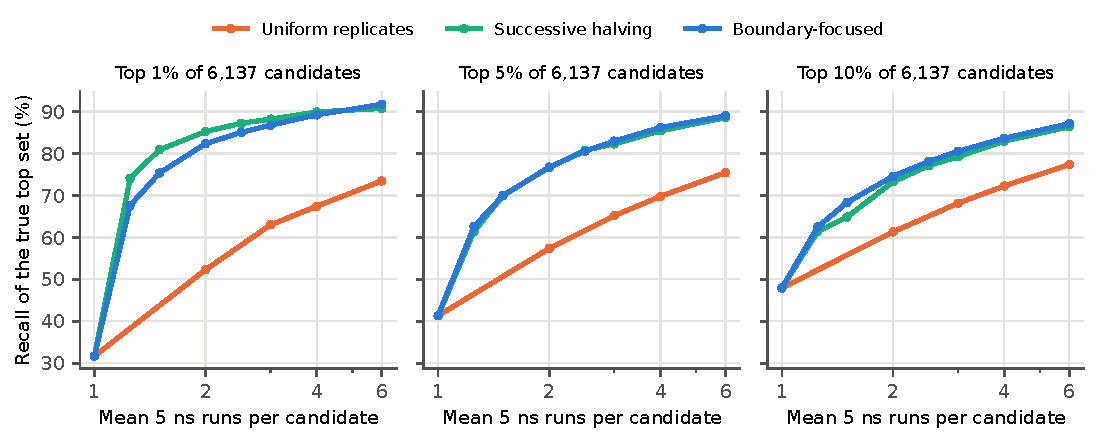
\includegraphics[width=\textwidth]{figures/fig8_allocation.pdf}
\caption{Recall of the true top set as a function of the mean number of \SI{5}{\nano\second} runs
per candidate, for three ways of allocating the budget (\alReps{} simulated campaigns of \alN{}
candidates with the measured noise; each run starts from a new, equilibrated structure). The
true top set is the top $k$ by the expected \SI{5}{\nano\second} label of each system, not by its
long-time diffusivity.}\label{fig:allocation}
\end{figure}


\subsection{A second property: the anion diffusivity}\label{sec:res-general}
To test whether these conclusions depend on the property, we repeated the main analyses for the
diffusivity of the TFSI anion (\cref{tab:general}). Because the platform distributes only the
origin-averaged estimate for the anion, both ions are compared with that estimator. The anion
label is much less noisy: its reliability is \genTfsiRel{} (95\% interval \genTfsiRelLo{} to
\genTfsiRelHi) against \genLiRel{} for lithium, so its noise ceiling is higher (\genTfsiCeil{}
against \genLiCeil) and a short run ranks the screening polymers better against the long runs
(Spearman \genTfsiRhoScreen{} against \genLiRhoScreen). The structure of the results, however, is
the same. The random forest comes close to the ceiling for both ions (\genTfsiMl{} and \genLiMl), its
correlation with the mean of two replicas rises as the measurement model predicts (\genTfsiMlMean{}
against an expected \genTfsiMlMeanExp{} for the anion), and adaptive allocation matches four
uniform replicates with less than half the runs ($\times$\genTfsiSaving{} and
$\times$\genLiSaving{} for the top 10\%). The numbers are specific to each property, but for these two properties the
conclusions are the same.

\begin{table}[ht]
\centering
\caption{Main results for the lithium and the TFSI anion diffusivities, both with the
origin-averaged estimator at half the run length. Noise statistics from the \nRep{} replicated
systems; random forest and allocation as in the previous sections (allocation with constant
noise).}\label{tab:general}
% Generado por generalidad.py. No editar a mano.
\begin{tabular}{lrr}
\toprule
 & \Li{} & TFSI$^-$ \\
\midrule
Run-to-run noise (log) & 0.28 & 0.19 \\
Noise, slow / fast half & 0.29 / 0.26 & 0.20 / 0.18 \\
Reliability (95\% CI) & 0.58 (0.44 to 0.70) & 0.80 (0.75 to 0.85) \\
Noise ceiling & 0.76 & 0.89 \\
Random forest vs one label & 0.77 & 0.86 \\
Random forest vs two-run mean (expected) & 0.84 (0.86) & 0.90 (0.90) \\
Spearman with 50 ns run, screening & 0.70 & 0.83 \\
Spearman with 50 ns run, literature & 0.94 & 0.96 \\
Runs matching 4 uniform replicates (top 10\%) & 1.7 ($\times$2.3) & 1.5 ($\times$2.7) \\
\bottomrule
\end{tabular}

\end{table}

\subsection{Practical guidance}\label{sec:res-guide}
\Cref{tab:guide} turns these results into recommendations, ordered from the least to the most
demanding purpose. They apply to the setting studied (LiTFSI in amorphous polymers, PCFF+,
\SI{353}{\kelvin}); the lengths are those for which this study provides evidence, not universal
minima. Five recommendations hold for every purpose: check that the potential energy has stopped
drifting before production starts, report the lag and the estimator of any
transport label together with the effective exponent of the population, prefer origin-averaged
estimates to end-point ones, never read a within-run error bar as the distance to the long-time
value, and remember that a lithium self-diffusivity ranks mobility, not conductivity: ion pairs
and clusters that move together raise $\Dapp$ without carrying net
charge~\cite{FranceLanord2019NernstEinstein}, so candidates selected by it should be checked for
ion correlations and transference number before they are called good electrolytes.

\begin{table}[ht]
\centering
\caption{Decision guide for MD screening, from the results of this study.}
\label{tab:guide}
\footnotesize\linespread{1.0}\selectfont
\begin{tabular}{@{}>{\raggedright\arraybackslash}p{0.19\textwidth}>{\raggedright\arraybackslash}p{0.24\textwidth}>{\raggedright\arraybackslash}p{0.49\textwidth}@{}}
\toprule
Purpose & What to do & Evidence in this study \\
\midrule
Separate good from poor candidates &
One \SI{5}{\nano\second} run each; rank by origin-averaged $\Dapp$ &
Spearman \PairAvgRhoLit{} among widely different polymers but \PairAvgRhoScreen{} among similar
screening polymers (origin-averaged estimator); not for fine ranking \\
\addlinespace
Find the best candidates under a fixed budget &
One run each, then new-structure replicates for candidates near the cut-off; with few rounds
available, one re-screening round of a shortlist &
In simulations with the measured noise, boundary-focused allocation matches four uniform
replicates with \alEqTopTenUnifFour{} runs per candidate for the top 10\% and
\alEqTopOneUnifFour{} for the top 1\% (\alRoundsTopTen{} and \alRoundsTopOne{} rounds); a single
re-screening round of a shortlist of $4k$ fixed in advance saves $\times$\alTwoStageFourkSavingTopTen{} and
$\times$\alTwoStageFourkSavingTopOne;
real runs consistent but underpowered \\
\addlinespace
Decide between two similar candidates &
Several new-structure runs each &
One run each: noise alone gives differences of $\times$\RepEndPairFactor{} (1 SD) and up to
$\times$\RepEndPairFactorNinetyFive{} (95\%) \\
\addlinespace
Train or evaluate a model on screening labels &
Split by system; average replicates where available; compare test metrics with the ceiling &
Correlation with single labels capped near \techoEndCorr{} (95\% CI \techoEndCorrLo{} to
\techoEndCorrHi); a fingerprint random forest reaches \mlCorr, and \mlRepMean{} against the mean of
two runs; improvements by better models are easier to demonstrate against averaged labels \\
\addlinespace
Estimate the apparent diffusivity at a stated lag &
5 to \SI{10}{\nano\second} with power-law extrapolation, one step above the cheapest setting &
Typical error \prePowErrFive{} from \SI{5}{\nano\second} against \preFitErrFive{} for a linear
fit; an empirical estimate at that lag, not of the long-time coefficient (underestimates the late
MSD slope) \\
\addlinespace
Obtain a diffusion coefficient or compare with experiment &
Simulate until the exponent is compatible with one and $\Dapp$ is flat across lag windows &
\betaLongDiffN{} of \nLong{} runs of \SI{50}{\nano\second} meet the criterion \\
\bottomrule
\end{tabular}
\end{table}

\subsection{Limitations}\label{sec:limitations}
All systems share one force field, one temperature and one salt; the conclusions hold for two
properties, the lithium and anion diffusivities, but other properties, such as the conductivity,
may have different noise. The long runs were chosen by
the dataset's authors rather than at random. The reference lag of \SI{25}{\nano\second} is not a
converged limit and shares data with the truncated trajectories, so prefix-based errors at long
$T$ are optimistic. Self-diffusion is a proxy for conductivity, which also depends on ion
correlations~\cite{FranceLanord2019NernstEinstein}, and finite-size
effects~\cite{Yeh2004SystemSize} are not corrected. The boxes are small (\tamBoxMin{} to
\SI{\tamBoxMax}{\nano\metre} side, \tamChainsMin{} to \tamChainsMax{} chains), so each
initial structure samples few chain conformations and packings; the structural part of the noise
may be smaller in larger boxes, which would raise the reliability of a single run. The noise model rests on \nRep{} replicated
pairs: the allocation gains are predictions of a model that the real runs, with \valAlNCamp{} systems,
do not contradict but cannot confirm; a campaign with several replicates per candidate would test
them directly. The analysis is largely exploratory: windows, thresholds, estimators and strategies
were compared on the same data, and only the stopping-rule settings were chosen and evaluated on
separate halves of the systems.

% =============================================================================
\section{Conclusions}\label{sec:conclusion}
% =============================================================================
Short MD runs provide useful screening labels, but those labels are both time dependent and noisy.
Across this collection, lithium mobility decreases during a run, together with that of the
polymer, while the system is still relaxing, so a \SI{5}{\nano\second} label
can overstate later-time mobility. Run-to-run noise accounts for about half of the variation
across candidates, with comparable contributions from initial structure and dynamics. This noise
limits prediction against single-run labels; the fingerprint model already approaches that limit,
and one run is better at separating very different polymers than ranking similar candidates.
Simulations with the measured noise suggest a practical allocation: run each candidate once, then
replicate candidates whose selection status is uncertain. This strategy can match four uniform
replicates at half the cost or less, although the real-run check is too small to confirm the gain.
A single re-screening round retains much of the saving, while adaptive stopping within individual
runs does not improve on fixed-length runs. The anion diffusivity shows a similar pattern, with
less noisy labels. For most systems, even runs ten times longer do not establish a long-time
transport coefficient.

% =============================================================================
\section*{Data and Software Availability}
The HTP-MD trajectories and curves are publicly available from the Toyota Research Institute
platform~\cite{Xie2023HTPMD}. The analysis scripts, the per-trajectory result tables and the
scripts that generate every number, table and figure of this paper are available at
\url{https://github.com/fhernandogallego/md-label-reliability} and archived on Zenodo
(\url{https://doi.org/10.5281/zenodo.23483460}); the raw trajectories are not redistributed.

\begin{suppinfo}
Data set details and validation of the trajectory processing; sensitivity of the regime census and
of the lag dependence; run-to-run reproducibility; end-point estimator; paired runs; prefix-based
estimators, stopping rules and held-out evaluation; robustness of the adaptive allocation and its check on real runs (PDF).
\end{suppinfo}

\begin{acknowledgement}
The authors acknowledge SCAYLE (Supercomputaci\'on Castilla y Le\'on, Le\'on, Spain) for
providing access to its computing infrastructure. This research received no external funding.
During the preparation of this work the authors used Claude (Anthropic) to assist with writing and
editing the manuscript, as none of the authors is a native English speaker, and to assist with
writing the analysis scripts. The authors designed the study, reviewed and verified all code,
results and text, and take full responsibility for the content of the publication.
\end{acknowledgement}

\section*{Notes}
The authors declare no competing financial interest.

\bibliography{references}

\end{document}

